%%%%%%%%%%%%%%%%%%%%%%%%%%%%%%%%%%%%%%%%%
% University/School Laboratory Report
% LaTeX Template
% Version 3.1 (25/3/14)
%
% This template has been downloaded from:
% http://www.LaTeXTemplates.com
%
% Original author:
% Linux and Unix Users Group at Virginia Tech Wiki 
% (https://vtluug.org/wiki/Example_LaTeX_chem_lab_report)
%
% License:
% CC BY-NC-SA 3.0 (http://creativecommons.org/licenses/by-nc-sa/3.0/)
%
%%%%%%%%%%%%%%%%%%%%%%%%%%%%%%%%%%%%%%%%%

%----------------------------------------------------------------------------------------
%	PACKAGES AND DOCUMENT CONFIGURATIONS
%----------------------------------------------------------------------------------------

\documentclass{article}

\usepackage[version=3]{mhchem} % Package for chemical equation typesetting
\usepackage{siunitx} % Provides the \SI{}{} and \si{} command for typesetting SI units
\usepackage{graphicx} % Required for the inclusion of images
%\usepackage{natbib} % Required to change bibliography style to APA
\usepackage{amsmath} % Required for some math elements 

\setlength\parindent{0pt} % Removes all indentation from paragraphs

%\renewcommand{\labelenumi}{\alph{enumi}.} % Make numbering in the enumerate environment by letter rather than number (e.g. section 6)

%\usepackage{times} % Uncomment to use the Times New Roman font

%----------------------------------------------------------------------------------------
%	DOCUMENT INFORMATION
%----------------------------------------------------------------------------------------

\title{PCR Detection of Genetically Modified Foods\\ AS.020.154: General Biology II Lab \\ Lab Report} % Title

\author{Indigo V. L. \textsc{Rose}} % Author name

\date{\today} % Date for the report

\begin{document}

\maketitle % Insert the title, author and date
\begin{center}
\textsc{Johns Hopkins University} \\ % Your university, school and/or department name(s)
\end{center}

\begin{center}
\begin{tabular}{l r}
Date Performed: & March 4, 2015 \\ % Date the experiment was performed
TA: & Elliot Turkiew \\ % TA
Partners: & Jonathan Martinez \\ % Partner names
& Priscilla Yan \\
Instructors: &  Rebecca Pearlman \\ % Instructor/supervisor
& Ami Patel
\end{tabular}
\end{center}

% If you wish to include an abstract, uncomment the lines below
% \begin{abstract}
% Abstract text
% \end{abstract}

%----------------------------------------------------------------------------------------
%	SECTION 1
%----------------------------------------------------------------------------------------

\section{Introduction}

This experiment utilized the polymerase chain reaction (PCR) technique to detect the presence of foreign DNA in several samples of food. Specifically, samples were tested for the presence of the 35S promotor from the \textit{Cauliflower mosaic virus} (CaMV-35S). This promotor is widely used in genetic engineering to insert desired genes into organisms by piggybacking on the virus' ability to easily insert its genome into the genomes of its target organisms [3]. If present, the 35S promotor is a strong indication that an organism has been genetically modified [2], [4]. \\
\\
Two control samples were used along with three test samples. The positive control was Quaker\texttrademark \ brand cornmeal, which is known to use CaMV-35S to insert exogenous DNA. An organic cornmeal known to be free of genetic engineering was used as a negative control. Samples taken from corn, blueberries, and Lay's\texttrademark \ brand potato chips were tested for evidence of this method of genetic modification. \\
\\
The blueberries were hypothesized to be free of the CaMV-35S promotor, as there are no known varieties of transgenic blueberries. While there are known varieties of engineered potatoes, the potato chips were hypothesized to also be CaMV-35S-free, as Frito-Lay issued a statement saying that it was not planning on using genetically modified ingredients [1]. The corn, on the other hand, was taken from an on-campus dining hall at Johns Hopkins University and its supplier was unknown. Many forms of genetically engineered corn exist[4], but it was unclear whether this was a transgenic variety. 

%----------------------------------------------------------------------------------------
%	SECTION 2
%----------------------------------------------------------------------------------------

\section{Materials and Methods}

In this experiment, DNA was extracted from several samples, and PCRed to test for the presence of the promotor described above. The materials and methods were followed closely from the General Biology II Lab course manual [4], which details each step and the specificities of the process in great detail. \\
\\
Two extraction techniques were utilized in the isolation of DNA from the three samples and two controls\textemdash one for hydrated foods and one for dried foods. The dried food method was used for the Lay's\texttrademark \  potato chips and the two controls, both dried cornmeal. The hydrated food method was used for the wet blueberries and wet corn. \\
\\
SYBR-Safe DNA stain was used in the agarose gel, instead of the ethidium bromide as described in the manual. The gel ran for about 60 minutes at 100 V.
%Note: The student does NOT need to rewrite all the steps of the experiment here. It is sufficient to cite the General Biology II Lab Manual. The student just needs to explain what he/she tested, and which method (?dry food? or ?wet food?) was used for each sample.
%Was the Materials and Methods section written in passive voice and past tense? (Example: ?Six samples were tested in this experiment. These include...?)
%Were any deviations from the protocol described? (Example: ?The samples were incubated at 65 degrees instead of at 60 degrees...?)

%----------------------------------------------------------------------------------------
%	SECTION 3
%----------------------------------------------------------------------------------------

\section{Results}

The PCR of the test samples appeared to have run relatively well and these data are displayed in Figure 1. The image showed no significant stripes at the region of interest (0.195 kB) for any of the three test samples. However, the controls worked only somewhat well: the region of interest lit up brightly for the positive control, but also dimly for the negative control. The blank worked well, showing an absence of any stripes, except for the haze of the primer dimer at the bottom. Perhaps problematic is that the blueberry lane is nearly devoid of fluorescence.\\
\\
The results of this experiment are summarized by Figure 1. A comprehensive table of the abbreviations used in the image are below. \\
\\
\begin{tabular}{l l l}
Abbreviation: & Lane: & Contents: \\
\hline
L & Lane 1 & DNA Ladder \\
B & Lane 2 & Blank (No DNA) \\
$+$ & Lane 3 & Quaker cornmeal \\
$-$ & Lane 5 & Organic cornmeal \\
Sample 1 & Lane 7 & Lay's potato chips \\
Sample 2 & Lane 9 & Corn \\
Sample 3 & Lane 11 & Blueberries \\
\end{tabular}
\\
% Image of gel
\begin{figure}[h]
\begin{center}
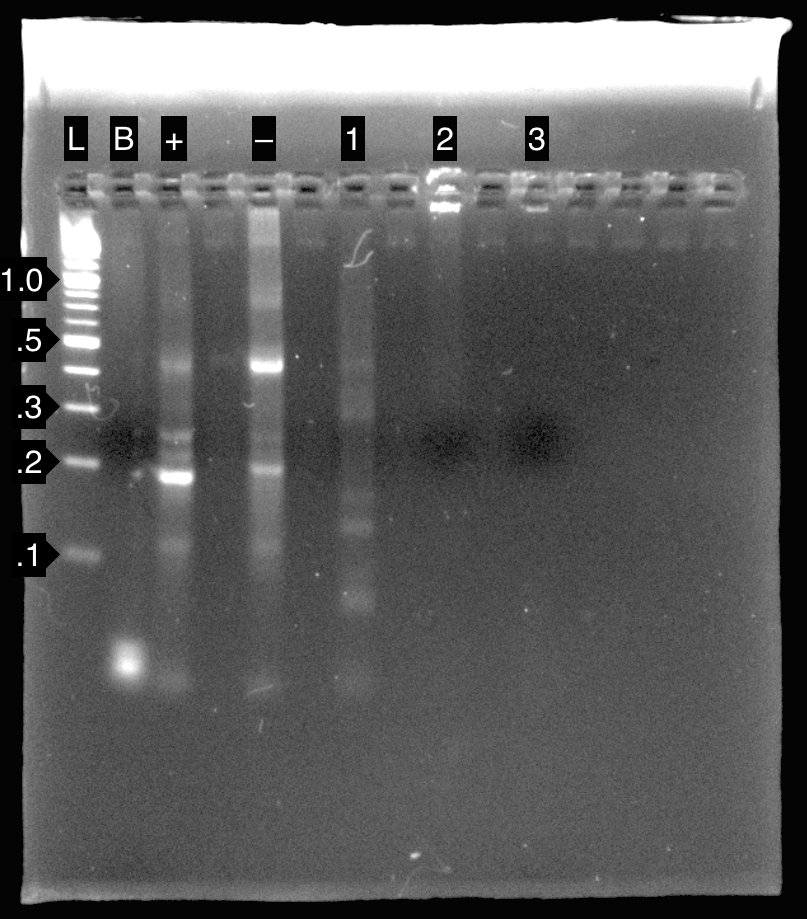
\includegraphics[width=0.77\textwidth]{M6gel} % Include the image placeholder.png
\caption{Agarose gel imaged under UV light to display florescence of dye bound to DNA. The numbers on the left side refer to the bands on the DNA ladder; they are measured in kilo-basepairs (kB). The contrast and exposure of this image were slightly increased from its original form in order to highlight the results.}
\end{center}
\end{figure}

%Did the student include a well-labeled electronic photograph of the gel?
%Did the photograph have a figure number, title, and caption? (Example: ?Figure 1: Agarose Gel. This gel was electrophoresed at XX volts...?)
%Was the figure mentioned in the text of the Results? (Example: ?As shown in Figure 1, the 2% sample....?)
%Is there text in the Results section BESIDES the text in the caption of the figure?
%Was the student careful not to make any conclusions about the results (saving them instead for the Discussion)?


%----------------------------------------------------------------------------------------
%	SECTION 4
%----------------------------------------------------------------------------------------
\pagebreak

\section{Discussion}

The results in Figure 1 indicate that none of the three test samples were found to contain the CaMV-35S promotor usually characteristic of genetically modified plants. This is inline with the hypothesized notions that the potato chips and blueberries didn't use this kind of genetic engineering, but it confirms that this is also true for the corn sample taken from an on-campus dining hall. While this does not prove that these foods haven't been genetically modified, it rules out the most commonly used method for doing so [4]. However, because of the presence of a light band on the negative control around 0.2 kB, any positive result might not be valid, but because all the results were negative, it's clear that there was no contamination from the Quaker cornmeal to Samples 1, 2, or 3.\\
\\
Some ambiguities in the experiment include the elusiveness of the blueberry sample on the agarose gel image and the band near 0.2 kB on the organic sample (negative control). It's difficult to determine if the blueberry sample (Sample 3) ran as intended. It's possible it did so just fine and that it's difficult to see it because of the low fluorescence or poor lighting in its specific lane. Alternatively, it's possible that a mistake was made and either its DNA wasn't properly extracted or its sample was mixed wrong, causing it not to run as intended. For the organic sample, it's probable that there was some DNA contamination from the Quaker sample, or it's possible that the organic cornmeal wasn't as so transgenic-free as originally thought.\\
\\
Further improvements on this experiment would include testing multiple negative controls to be sure of their authenticity as well as testing multiple trials of each sample, especially the blueberries, to gain more confidence in the results. 
%Did the student make appropriate conclusions about the results?
%If the results were unclear or not what was expected, did the student discuss possible causes?
%Did the student discuss ideas for further experiments related to this one?

%----------------------------------------------------------------------------------------
%	SECTION 5
%----------------------------------------------------------------------------------------

\section*{References}

\begin{description}
   \item[1.] Charles, D. (2015, January 15). GMO Potatoes Have Arrived. But Will Anyone Buy Them? Retrieved April 6, 2015, from http://www.npr.org/ blogs/thesalt/2015/01/13/376184710/gmo-potatoes-have-arrived-but-will-anyone-buy-them

   \item[2.] DG JRC (1998). Directorate Generals European Commissions Joint Research Centre, Environment Institute, Consumer Protection \& Food Unit. Screening method for the identification of genetically modified organisms (GMO) in food.

   \item[3.] Hull, R., Covey, S., \& Dale, P. (2000). Genetically modified plants and the 35S promoter: Assessing the risks and enhancing the debate. \textit{Microbial Ecology in Health and Disease}.
 
   \item[4.] PCR Detection of Genetically Modified Foods: Electrophoresis [Class Handout]. (2015). Baltimore, MD: Johns Hopkins University.
   
\end{description}



%\begin{thebibliography}{1}

%\end{thebibliography} 


%----------------------------------------------------------------------------------------
%	BIBLIOGRAPHY
%----------------------------------------------------------------------------------------

%\bibliographystyle{apalike}
 

%\bibliography{sample}

%----------------------------------------------------------------------------------------


\end{document}